\subsection{Database}
Denne section beskriver design og implementering af database delen som er lavet på baggrund af kravspecifikationen og systemarkitekturen.\\
Databasen er blevet opdelt i 2 dele som håndtere denne side. Databasen er opdelt i serveren og web-siden.
\begin{figure}[H]
\centering
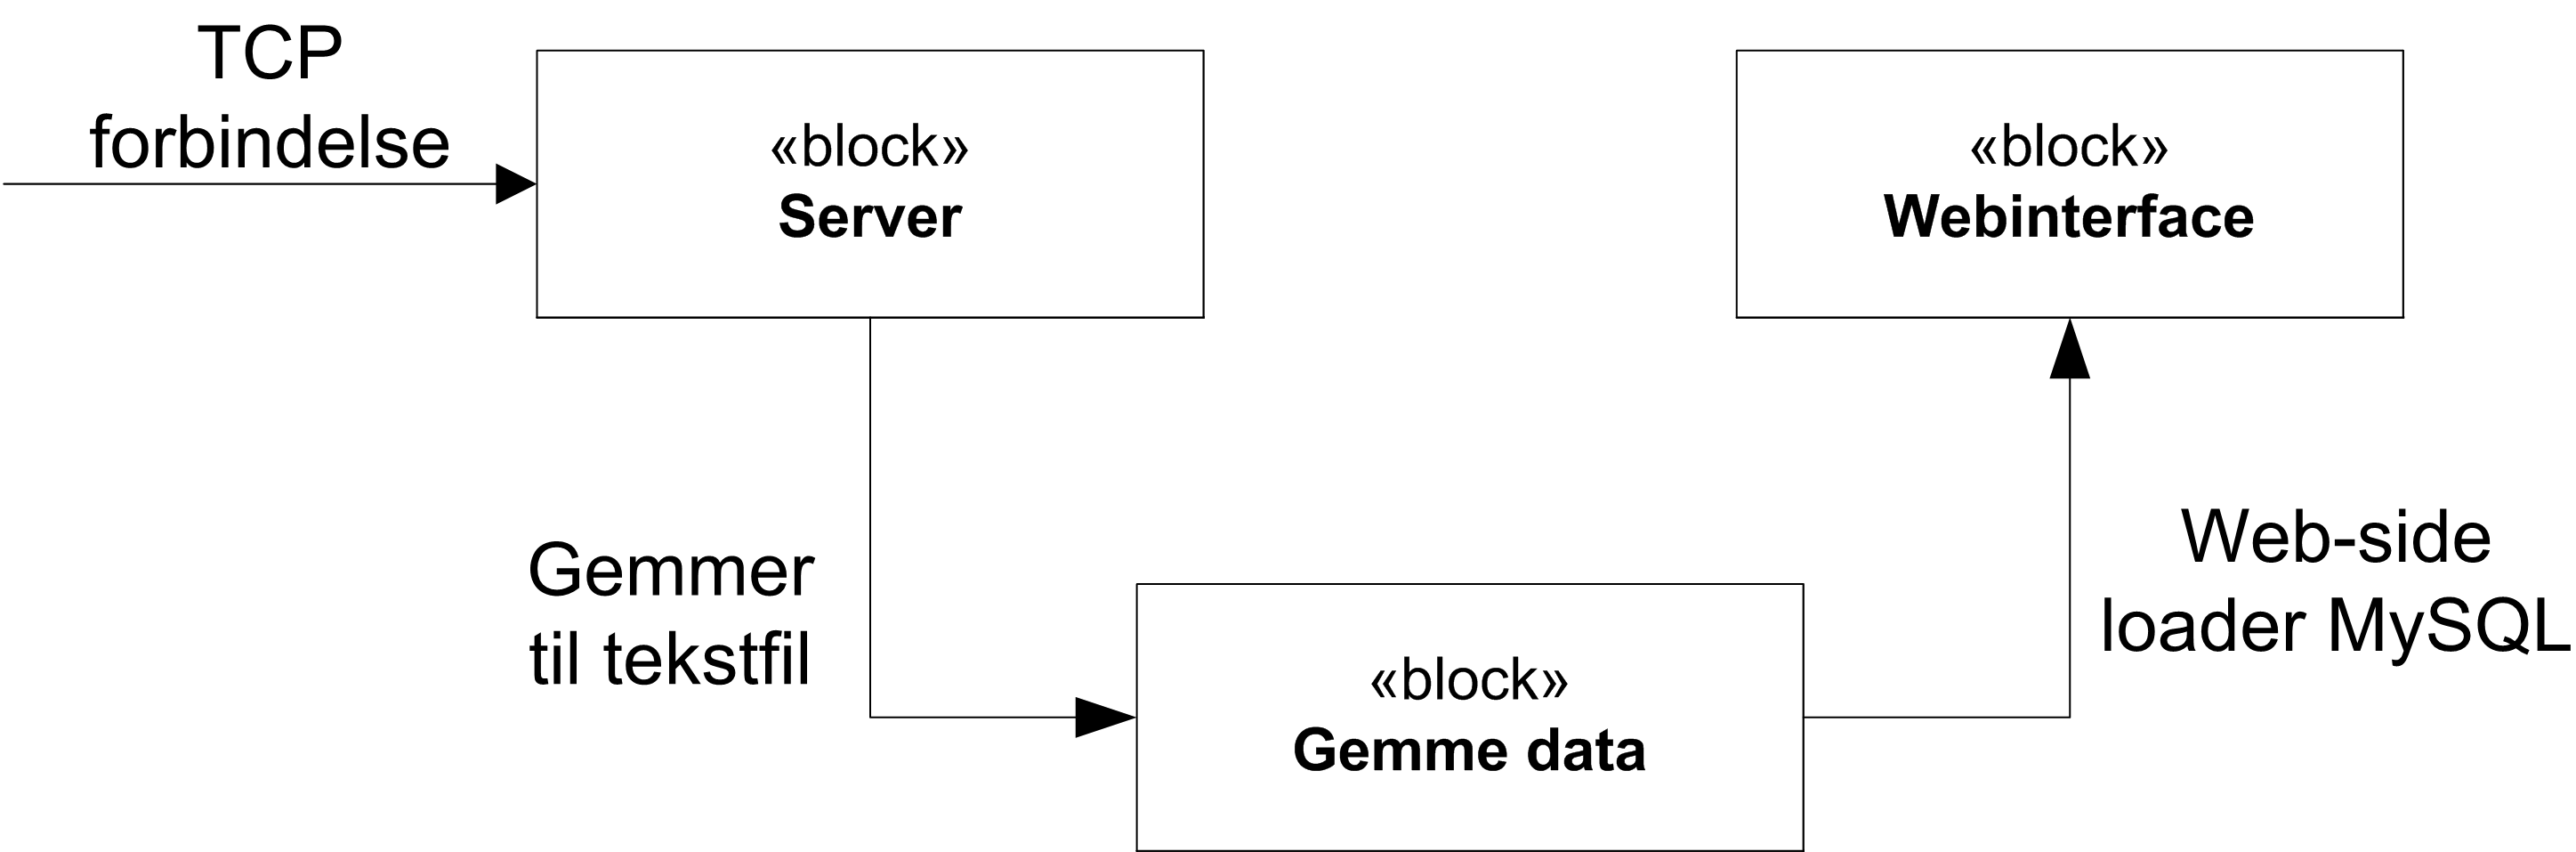
\includegraphics[width = 0.5\textwidth]{billeder/database_to_mysql}
\caption{Illustrere overordnet hvordan databasen fungere}
\label{fig:server_to_mysql}
\end{figure}

\subsection{Serveren}
Denne section beskriver design og implementering af serveren.
Opbygningen af severen er gjort i klasser sådan at hver element i severen er implementeret som en klasse se figur \ref{fig:database_server}. Ud over dette benyttes der nogle hjælpeklasser.\\

Det gælder at når KI forsøger at kontakte databasen, tilsluttes denne via tcp som benytter sig af socket. Når tilslutningen er gjort kan der overføres data fra KI til databasen. Dataerne bliver gemt i mySQL databasen. I tilfælde af at der blvier problermer med at gemme, laves der en en tekst fil hvori dataerne bliver lagt og kan så forsøgt gemt af web siden.
\begin{figure}[H]
\centering
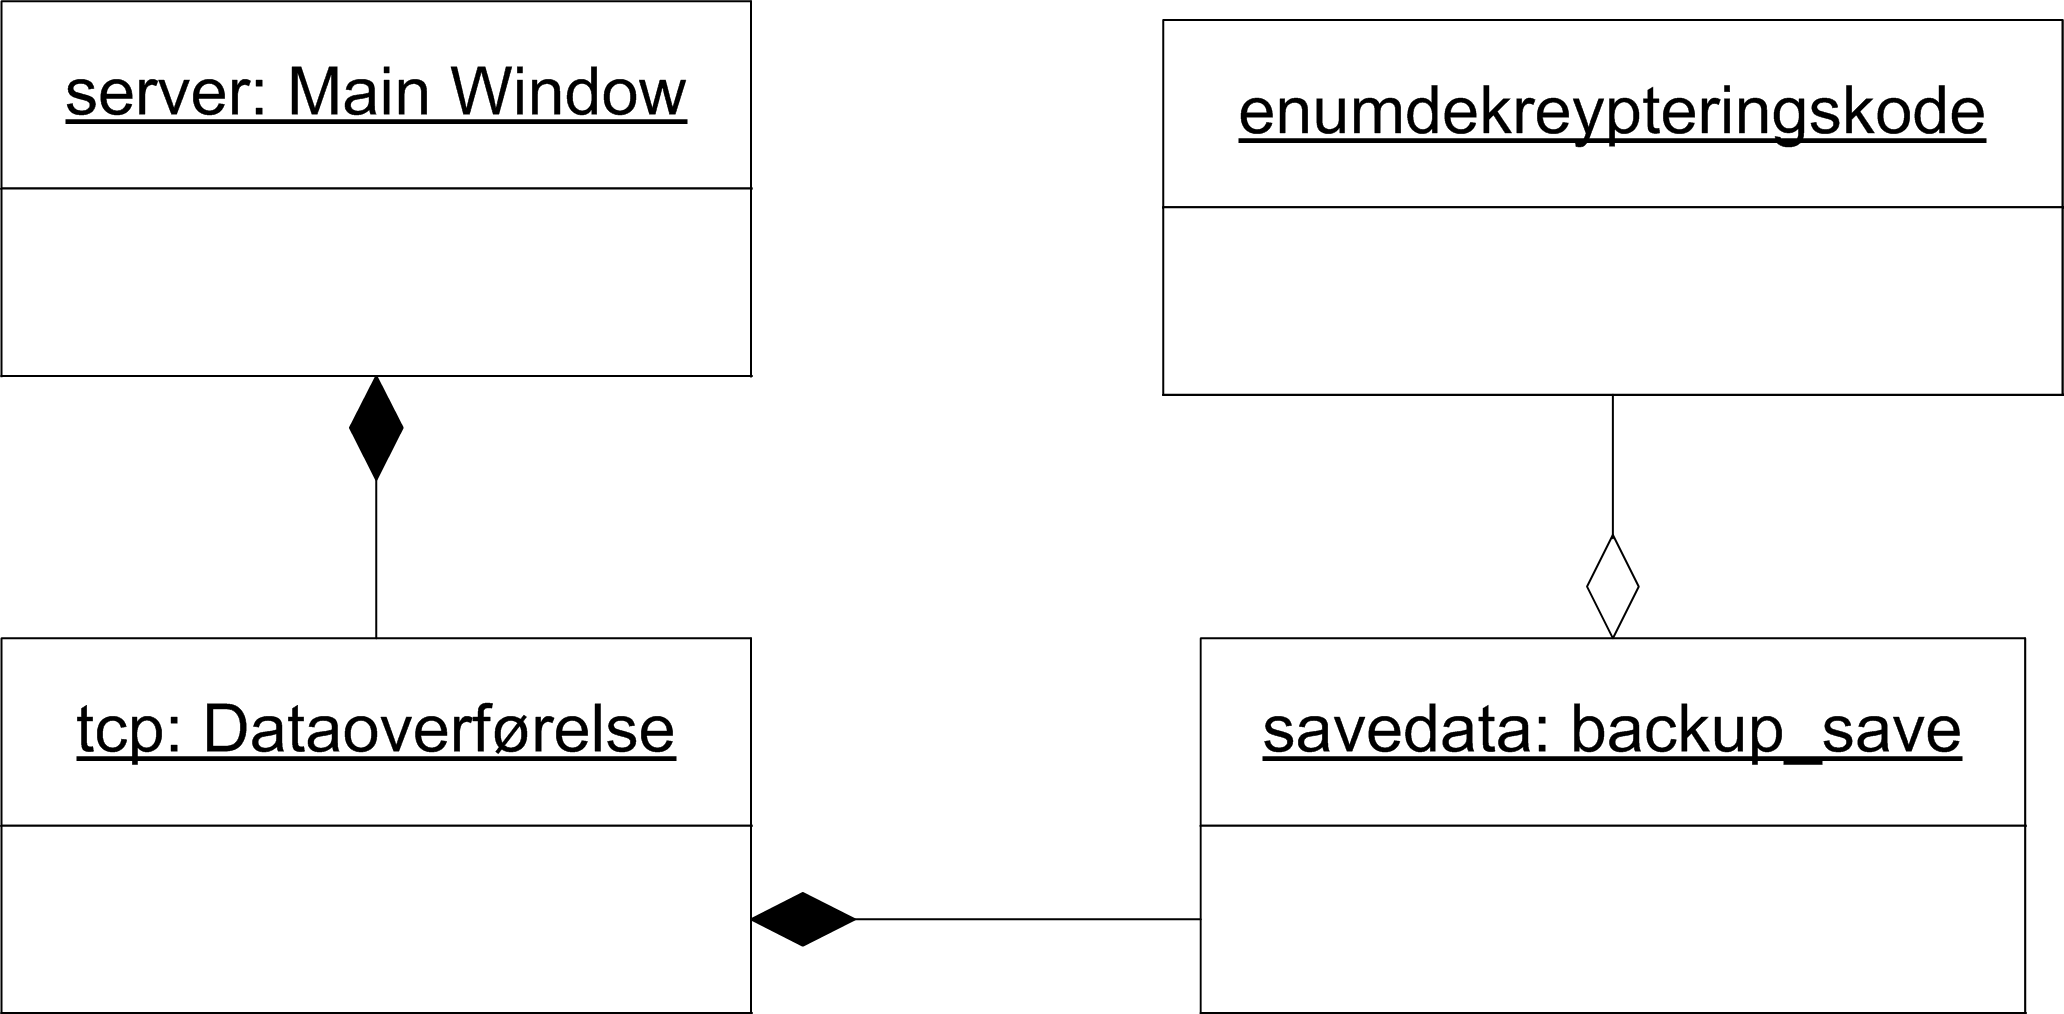
\includegraphics[width = 0.5\textwidth]{billeder/database_server}
\caption{Illustrere overordnet hvordan serveren fungere}
\label{fig:database_server}
\end{figure}

\begin{table}[H]
\centering
\begin{tabular}{p{3cm} p{12.5cm}}
\multicolumn{2}{l}{{\Large Serverens klasser}} \\\hline
Server & Er hovedvinduet på serveren. Information til brugeren udskrives herfra og knapper er implementeret. \\
TCP forbindelse (tcp) & Opretter en mulig tcp forbindelse hvor skibet kan tilslutte sig og overføre data.\\
Gemme data (savedata) & Gemmer data til en tekst fil hvis ikke det har været muligt for serveren at få kontakt til mySQL.\\
De kryptering(enumDeKrypteringskode) & Dekryptere level fra sm så data bliver i grader\\
\end{tabular}
\caption{Serverens klasser}
\label{tabel:server-klasser}
\end{table}

\subsection{Web-side}
Denne section beskriver design og implementering af web siden.\\
Opbygningen af web siden er gjort hovedsageligt i php hvor dette gav mening. Desuden er html og styles (css) blevet benyttet til at sikre ens stil på hele web siden og for simpelt at kunne veligeholdes. For at sikre mindst data transmision imellem computer og server er princippet i ajax blevet benyttet.

Når havneterminalen ønsker at se data om skibe der er opkoblet på BROS kan denne tilgå disse via den web baserede database. Når serveren køre kan brugeren tilgå databasen via knappen "Database" ellers kan denne tilgås via den locale adresse. For at komme ind i databasen skal brugeren taste sit password dette gøres for at sikre imod uaotirseret brug af databasen. Efter log ind på siden kan brugeren vælge hvilket skib der skal benyttes. Når skib er valgt komemr brugeren ind på den valgte database. Her kan brugeren se ID på skibet vandtilstand i ballast tanke, hældning og tid siden sidste opdatering (for nærmere se apandix\fxnote{link til apendix}). Hvis serveren har haft problemer med at gemme den nyeste data vil web siden forsøge at gemme som det første inden databasen loades. 

\begin{figure}[H]
\centering
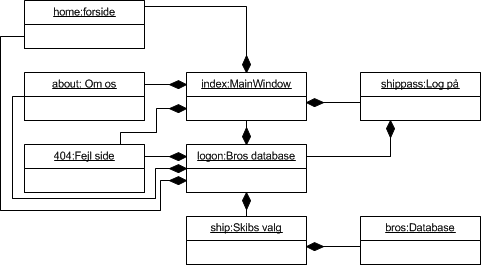
\includegraphics[width = 0.5\textwidth]{billeder/database_web}
\caption{Illustrere overordnet hvordan web-siden fungere}
\label{fig:database_web}
\end{figure}

\begin{table}[H]
\centering
\begin{tabular}{p{3cm} p{12.5cm}}
\multicolumn{2}{l}{{\Large Web sidens beskrivelse}} \\\hline
Hovedvindue (index) & Den første side brugeren kommer til om ikke denne går via serveren \ref{tabel:server-klasser} Denne side loader siden Forside, Om os og Log in ind i sig.\\
Databasen (logon) & Denne side bliver kaldt efter at brugeren er logget på. Denne side loader Skibs valg, bros datasen for skibet, Forside og Om os. 
\end{tabular}
\caption{Web sidens opbygning}
\label{tabel:webside-simpel}
\end{table}